\chapter{Analyse et spécification des besoins}
\label{chap:analyse_besoins}
\section*{Introduction}
\addcontentsline{toc}{section}{Introduction}
La spécification des besoins constitue une étape essentielle dans le développement d’un projet.
Elle permet de passer d’une vision abstraite du sujet à une définition concrète du produit,
en comprenant clairement le travail qui reste à faire. Cette étape est aujourd’hui d’autant plus
critique car elle doit piloter la rencontre entre la gestion des big data, le pilotage commercial
traditionnel et l’adjonction de solutions d’IA prédictives ou génératives dans le cadre de ce
projet de CRM smart avec moteur de lead scoring par IA.

Dans ce chapitre, nous commencerons par identifier les différents acteurs impliqués et leurs
rôles respectifs, puis nous déterminerons les exigences fonctionnelles et non fonctionnelles que
notre système doit répondre. Enfin, nous effectuerons une modélisation UML complète, struc-
turée par acteur et par cas d’utilisation précis, pour aboutir à une application qui réponde par-
faitement aux besoins des utilisateurs.

\section{Identification des acteurs}

Selon les formalismes UML, un acteur définit un rôle externe qui interagit avec le système
pour en obtenir une valeur ajoutée. Le cœur de notre CRM intelligent réside dans une synergie
entre des acteurs humains, avec des rôles hiérarchisés, et des services d’intelligence artificielle
qui améliorent l’expérience utilisateur.

\subsection*{Acteurs principaux}

\begin{itemize}
    \item \textbf{Sales Representative (Commercial)} : C’est l’acteur opérationnel au cœur du système.
    Sa mission consiste à convertir des opportunités commerciales potentielles en ventes
    réelles. Il se connecte à la plateforme pour voir et gérer ses leads assignés, piloter ses
    contacts et deals, planifier ses activités quotidiennes (appels, tâches, réunions) et utiliser
    les outils d’intelligence artificielle afin de personnaliser sa communication. Pour lui, le
    CRM devient un assistant proactif qui priorise son travail grâce au scoring prédictif et
    automatise ses rédactions grâce à l’IA Gemini.
    
    \item \textbf{Sales Manager / Administrateur} : Il intervient au plan stratégique et technique. Il
    est en charge de l’intégrité de la plateforme, de la gestion des comptes utilisateurs et
    de l’analyse des performances de l’ensemble de l’équipe commerciale. Il joue un rôle
    clé dans les phases de migration de données, orchestrant les modules d’importation de
    masse à partir de fichiers CSV. Il a également accès à toutes les analytics et les tableaux
    de bord, lui permettant d’adapter la stratégie commerciale en fonction des indicateurs
    donnés par le système.
\end{itemize}

\subsection*{Acteurs secondaires (Systèmes)}

Notre application repose sur des services externes dont les contrats d’interface donnent la possibilité de traiter et d’accéder aux données du système. Les systèmes utilisés sont les sui-
vants :

\begin{itemize}
    \item \textbf{Système Gemini API — Google} : Google Gemini (modèle gemini-1.5-flash) fonctionne comme un service de traitement du langage naturel (NLP) pour la génération automa-
    tique de contenu personnalisé. Ce service permet de rédiger des brouillons d’emails commerciaux adaptés en analysant les données contextuelles d’un prospect (notes, histo-
    rique d’emails, score IA, informations sur l’entreprise). De plus, il propulse un assistant conversationnel (Chatbot) intelligent qui utilise l’approche RAG (Retrieval-Augmented Generation) pour répondre en temps réel aux questions de l’utilisateur sur les données CRM.
    
    \item \textbf{Lead Scoring AI Agent (Micro-service FastAPI)} : C’est un micro-service Python conçu pour l’analyse prédictive, développé avec le framework FastAPI. Il offre l’endpoint \texttt{POST /predict-score} qui reçoit les caractéristiques comportementales et contex-
    tuelles d’un lead. Il renvoie un score de conversion sur 100 et une catégorie qualitative (Hot, Warm, ou Cold) produite par un modèle RandomForestClassifier entraîné.
    
    \item \textbf{Système de gestion de base de données MySQL} : C’est le système de gestion de base de données relationnelle qui garantit la persistance de toutes les données de l’application. Ce système est géré grâce à l’ORM Prisma, qui assure la protection des requêtes et l’uniformité du schéma de données.
\end{itemize}

\section{Spécification des besoins}

Cette section vise à rassembler, examiner et établir les besoins fondamentaux et les caracté-
ristiques du projet. Elle met l’accent sur les besoins fonctionnels et non fonctionnels indispen-
sables pour offrir des services simples à utiliser et à entretenir.

\subsection{Les besoins fonctionnels}

Les exigences fonctionnelles définissent les attentes de chaque intervenant concernant l’ap-
plication à concevoir. Dans le contexte de notre projet, nous avons repéré les exigences fonc-
tionnelles qui suivent :

\begin{itemize}
    \item \textbf{Connexion} : L’utilisateur se connecte à l’application en entrant ses informations d’iden-
    tification (adresse électronique et mot de passe). Le système produit un jeton JWT si-
    gné qui permet l’accès aux ressources sécurisées en fonction du rôle de l’utilisateur, soit ADMIN ou REP.
    
    \item \textbf{Gestion des Prospects} : L’utilisateur a la possibilité de créer, visualiser, modifier et éliminer des prospects. Chaque piste est liée à une étape de cycle de vie (NOUVEAU, CONTACTÉ, QUALIFIÉ, PERDU), une estimation de la valeur de l’affaire, des rensei-
    gnements sur la société et un score IA qui est automatiquement calculé par le micro-
    service prédictif.
    
    \item \textbf{Vérification du Score IA d’un Lead} : L’utilisateur est en mesure de déclencher le calcul de la probabilité de conversion d’un lead. Le système sollicite le micro-service FastAPI par l’intermédiaire de \texttt{POST /predict-score} et présente la réponse sous la forme d’un score quantitatif (0-100) complété par une évaluation qualitative de la température (Hot/Warm/Cold) et une série d’arguments explicatifs.
    
    \item \textbf{Produire un courrier électronique grâce à l’IA (Gemini)} : L’utilisateur a la possibilité de solliciter la création d’un projet de courrier électronique sur mesure pour un prospect. Le système évalue le contexte du prospect et sollicite l’API Google Gemini afin de générer un contenu sur mesure. Si l’API n’est pas disponible, un système de règles fixes est utilisé en remplacement (on parle alors de « Graceful Degradation »).
    
    \item \textbf{Assistant conversationnel intelligent (RAG avec Gemini)} : L’utilisateur dispose d’un assistant virtuel (chatbot) pour interroger les données du CRM en langage naturel. Le backend NestJS extrait dynamiquement le contexte lié aux prospects, deals et statis-
    tiques globales depuis MySQL pour alimenter le modèle Gemini, permettant des ré-
    ponses ultra-ciblées sur les données réelles et empêchant les réponses aléatoires.
    
    \item \textbf{Administration des Contacts} : L’utilisateur a la possibilité de créer, visualiser, changer et effacer des contacts clients. Chaque contact est associé à une entreprise et peut être lié à de multiples pistes, activités et demandes d’assistance.
    
    \item \textbf{Administration des Entreprises (Companies)} : L’utilisateur a la possibilité de gérer l’inventaire des entreprises clients ou en perspective, comprenant leurs informations dé-
    taillées (domaine d’activité, dimension, site internet, pays).
    
    \item \textbf{Administration du Pipeline Commercial (Transactions)} : L’utilisateur a la possibi-
    lité d’établir et de suivre des prospects commerciaux via un pipeline de vente visuel en format Kanban. Chaque transaction est liée à une somme d’argent, une date de fin approximative et un état (PENDING, ACTIVE, WON, LOST).
    
    \item \textbf{Administration des Activités} : L’utilisateur a la possibilité de programmer et d’or-
    ganiser ses interactions professionnelles : appel téléphonique, envoi d’email, réunion ou tâche. Chaque action est associée à un prospect ou un contact et peut être indiquée comme terminée.
    
    \item \textbf{Administration des Billets de Support} : L’usager a la possibilité de générer des de-
    mandes d’assistance pour identifier et suivre les problèmes ou requêtes. Les tickets passent par une séquence de statuts (NEW, OPEN, PENDING, RESOLVED, CLOSED) et sont classés selon un niveau de priorité (LOW, MEDIUM, HIGH, CRITICAL).
    
    \item \textbf{Importation massive de données (CSV)} : Il est possible pour l’administrateur d’im-
    porter plus de 1 000 enregistrements (contacts, leads ou entreprises) à partir d’un fichier CSV. Le système valide chaque ligne, détecte les doublons par une clé composite (Email + UserId) et génère un rapport d’importation synthétique.
    
    \item \textbf{Accéder aux Tableaux de Bord et aux Analyses} : L’administrateur peut consulter des tableaux de bord dynamiques qui récapitulent les indicateurs clés de performance (KPIs) de l’équipe commerciale : le taux de transformation, la distribution des prospects selon leur statut, la valeur globale du pipeline et les résultats par représentant commercial.
    
    \item \textbf{Gestion des Comptes Utilisateurs} : L’administrateur a la possibilité de créer, changer, activer ou désactiver les comptes des membres de l’équipe, en leur attribuant le rôle adéquat.
    
    \item \textbf{Obtenir des Notifications} : L’utilisateur est averti en direct par le système lors d’évé-
    nements essentiels : l’arrivée d’un nouveau prospect prometteur, l’approche imminente d’une tâche, ou la mise à jour de la situation d’un ticket.
\end{itemize}

\subsection{Les besoins non fonctionnels}

Les exigences non fonctionnelles se referent aux besoins opérationnels qui définissent la
qualité du système. Pour notre application, nous avons défini et intégré les exigences non
fonctionnelles suivantes :

\subsubsection{A. Sécurité et Confidentialité}

La sécurité est une priorité absolue, particulièrement pour un CRM manipulant des données clients sensibles.

\begin{itemize}
    \item \textbf{Où et comment c’est intégré :}
    \begin{itemize}
        \item \textbf{Authentification} : Intégrée au niveau du backend (NestJS) via des jetons JWT sto-
        ckés et gérés par les Guards (ex. JwtAuthGuard) pour sécuriser les routes.
        \item \textbf{Autorisation (RBAC)} : Déployée à l’aide des décorateurs personnalisés (ex. décorateur \texttt{@Roles('ADMIN')} dans les contrôleurs NestJS) pour bloquer l’accès non autorisé aux routes critiques (comme l’import CSV ou la gestion de tous les comptes).
        \item \textbf{Isolation des données} : Implémentée dans les services (Services) via Prisma, où les requêtes SQL (ex. userId: req.user.id) filtrent systématiquement les entités (leads, contacts, deals) selon l’utilisateur connecté pour empêcher les accès croisés.
        \item \textbf{Chiffrement} : Utilisé lors de la création et de la mise à jour des mots de passe grâce à l’algorithme Bcrypt dans le module utilisateur.
    \end{itemize}
\end{itemize}

\subsubsection{B. Performance et Réactivité}

L’application doit répondre instantanément pour garantir la productivité des commerciaux.

\begin{itemize}
    \item \textbf{Où et comment c’est intégré :}
    \begin{itemize}
        \item \textbf{Rendu Frontend} : Utilisé de manière globale via le framework Next.js (App Rou-
        ter) qui pré-génère les pages côté serveur (SSR) et garantit des temps de chargement réduits.
        \item \textbf{Optimisation des bases de données} : Intégrée dans le schéma Prisma en définissant des index sur les clés étrangères pour accélérer les jointures. Par exemple : \texttt{@index([userId])} et \texttt{@index([companyId])}, ce qui améliore les performances lors de l’affichage des tableaux de bord analytiques complexes.
        \item \textbf{Mises à jour en temps réel (Triggers)} : Implémentées dans le frontend via les hooks useEffect qui "écoutent" les modifications d'état (ajout de notes, tâches complétées) pour re-fetcher dynamiquement les données statistiques sans rafraîchir la page.
    \end{itemize}
\end{itemize}

\subsubsection{C. Disponibilité, Résilience et Tolérance aux pannes}

Le CRM doit rester opérationnel même en cas de défaillance partielle des services tiers.

\begin{itemize}
    \item \textbf{Où et comment c’est intégré :}
    \begin{itemize}
        \item \textbf{Mécanisme de Fallback (Graceful Degradation)} : Intégré dans le service \texttt{ai-email.service} — si l’API Google Gemini échoue, un email générique est généré à partir de modèles locaux. De même, si le micro-service FastAPI ne répond pas, un algorithme de secours fondé sur des règles calcule un score de repli.
        \item \textbf{Gestion des erreurs globales} : Implémentée via des Exception Filters dans NestJS et des Toast Notifications (avec react-hot-toast) dans Next.js pour avertir l’utilisateur d’un problème sans faire crasher l’application logicielle.
    \end{itemize}
\end{itemize}

\subsubsection{D. Évolutivité et Scalabilité}

L’architecture doit pouvoir supporter une augmentation du nombre d’utilisateurs et de la quantité de données gérées.

\begin{itemize}
    \item \textbf{Où et comment c’est intégré :}
    \begin{itemize}
        \item \textbf{Architecture Micro-services} : Le découpage du projet en trois entités distinctes (Frontend Next.js, Backend NestJS, Agent IA FastAPI) permet d’allouer plus de ressources de manière granulaire, uniquement au service qui en a besoin (ex. scaler FastAPI lors d’un pic d’analyses prédictives).
        \item \textbf{Conteneurisation} : Utilisation de Docker (via les fichiers Dockerfile et docker-compose) pour garantir que chaque composant est isolé et peut être déployé ou mis à l’échelle sur le cloud sans conflit de dépendances.
    \end{itemize}
\end{itemize}

\subsubsection{E. Maintenabilité et Qualité du Code}

Le code doit être facilement compréhensible et modifiable par de nouveaux développeurs rejoignant le projet.

\begin{itemize}
    \item \textbf{Où et comment c’est intégré :}
    \begin{itemize}
        \item \textbf{Typage fort} : Application stricte de TypeScript partagée entre le frontend et le backend pour prévenir les anomalies au moment de la compilation.
        \item \textbf{Architecture Modulaire} : Implémentée dans NestJS à travers le concept de Modules (ex. LeadsModule, AnalyticsModule), en séparant très clairement les responsabilités MVC (Controllers, Services, DTOs).
        \item \textbf{ORM Centralisé} : L’utilisation du fichier schema.prisma qui agit comme source unique de vérité pour le modèle de données, facilitant la gestion des migrations lors de modifications de la base.
    \end{itemize}
\end{itemize}

\subsubsection{F. Ergonomie et Utilisabilité (UX/UI)}

Le système doit être intuitif, esthétique et facile à prendre en main pour réduire le temps de formation des utilisateurs commerciaux.

\begin{itemize}
    \item \textbf{Où et comment c’est intégré :}
    \begin{itemize}
        \item \textbf{Composants Visuels} : Construits dans l’interface utilisateur en exploitant le frame-
        work Tailwind CSS et les icônes de Lucide React pour une consistance visuelle moderne et compréhensible.
        \item \textbf{Comportement Réactif (Responsive)} : Le design des interfaces (Tableaux, Kan-
        bans, Modules de détails) est nativement conçu pour s’adapter et rester fonctionnel sur de multiples résolutions d’écran.
        \item \textbf{Feedback Visuel dynamique} : Application d’animations fluides lors d’actions clés (Drag \& Drop dans le Pipeline, micro-animations sur les graphiques analytiques) et de spinners de chargement lors d’appels asynchrones, rendant la plateforme "vi-
        vante".
    \end{itemize}
\end{itemize}

\subsubsection{G. Interopérabilité}

Le système doit être capable de communiquer de manière fluide et normée avec ses multiples services internes ou externes.

\begin{itemize}
    \item \textbf{Où et comment c’est intégré :}
    \begin{itemize}
        \item \textbf{Architecture API RESTful} : Le backend NestJS expose des points d’accès standards (endpoints) permettant au frontend de consommer les données de façon dé-
        couplée, facilitant la création éventuelle d’une future application mobile.
        \item \textbf{Protocoles Standardisés} : L’échange de données entre le backend principal et le micro-service d’Intelligence Artificielle (FastAPI) ainsi que les API externes (Google Gemini) se fait exclusivement en format JSON via HTTP, assurant une totale inter-
        opérabilité indépendamment des langages de programmation.
    \end{itemize}
\end{itemize}

\section{Diagrammes de cas d’utilisation}

Un diagramme de cas d’utilisation représente les fonctionnalités du système du point de vue de l’utilisateur et fournit une vision générale du comportement fonctionnel de l’application. La conceptualisation de ces diagrammes est une étape primordiale pour produire un logiciel conforme aux attentes des parties prenantes.

\subsection{Structuration en packages}

La structuration d’un modèle statique repose sur deux principes fondamentaux : la cohé-
rence et l’indépendance. Pour simplifier notre modèle, nous avons organisé les cas d’utilisation en les regroupant dans des ensembles fonctionnels cohérents, appelés packages, illustrés dans la figure 2.1.

\begin{figure}[H]
    \centering
     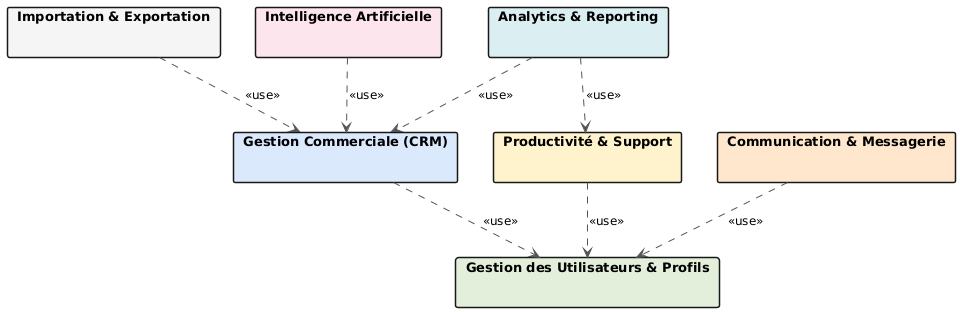
\includegraphics[width=0.85\textwidth]{images/packages_fonctionnels.png}
    \caption{Structuration en packages fonctionnels du système CRM}
    \label{fig:packages}
\end{figure}

\subsection{Diagramme de cas d’utilisation du côté « Sales Representative »}

Le diagramme de cas d’utilisation du côté « Sales Representative » est présenté ci-dessous dans la figure 2.2. Ce participant dispose d’un accès à l’ensemble des fonctionnalités du CRM indispensables pour mener à bien ses activités commerciales. Il communique directement avec deux systèmes externes : l’API Gemini pour la création d’emails, et le micro-service de notation IA pour juger ses prospects.

\begin{figure}[H]
    \centering
     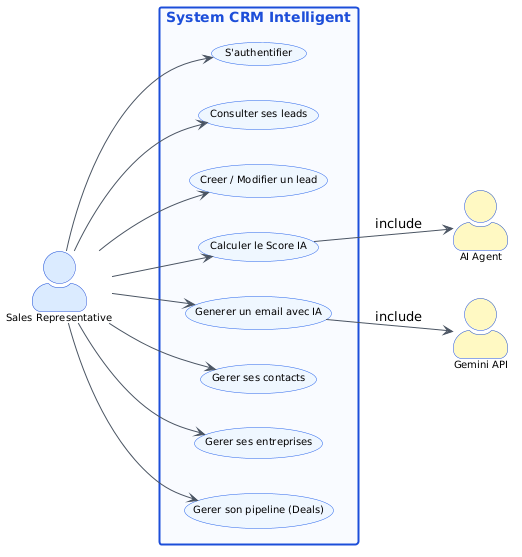
\includegraphics[width=0.9\textwidth]{images/uc_sales_rep.png}
    \caption{Diagramme de cas d’utilisation du côté « Sales Representative »}
    \label{fig:uc_sales_rep}
\end{figure}

\subsection{Diagramme de cas d’utilisation du côté « Administrateur »}

La figure 2.3 illustre les scénarios d’utilisation pour l’acteur « Administrateur / Sales Mana-
ger ». Outre les fonctionnalités opérationnelles disponibles pour le Représentant Commercial, l’administrateur a des privilèges uniques qui lui permettent de contrôler intégralement la plate-
forme : gestion des comptes, importation en grande quantité de données et accès à des analyses sophistiquées.

\begin{figure}[H]
    \centering
    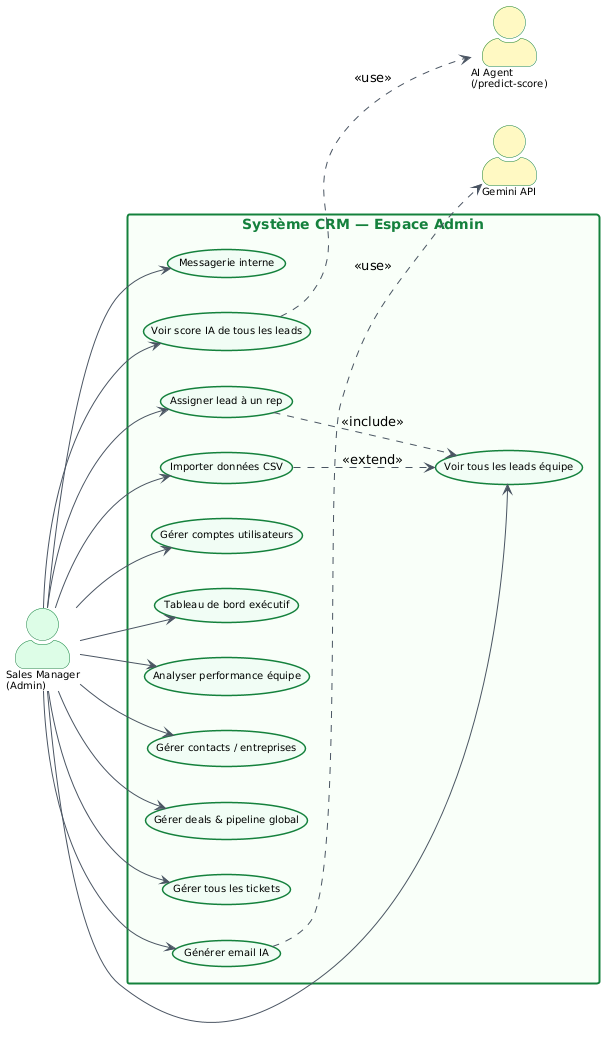
\includegraphics[width=0.9\textwidth]{images/uc_admin.png}
    \caption{Diagramme de cas d’utilisation du côté « Administrateur »}
    \label{fig:uc_admin}
\end{figure}

\subsection{Diagramme de cas d’utilisation relatif au cas d’utilisation « Gérer les Leads »}

Le diagramme de la figure 2.4, relatif au cas d’utilisation « Gérer les Leads », permet de visualiser de manière claire et concise les sous-cas d’utilisation associés. La gestion des leads englobe un cycle de vie complet allant de la création à la clôture, enrichi par les fonctionnalités d’intelligence artificielle. L’utilisateur peut créer un lead, mettre à jour son statut, consulter son score prédictif et générer un email personnalisé.

\begin{figure}[H]
    \centering
     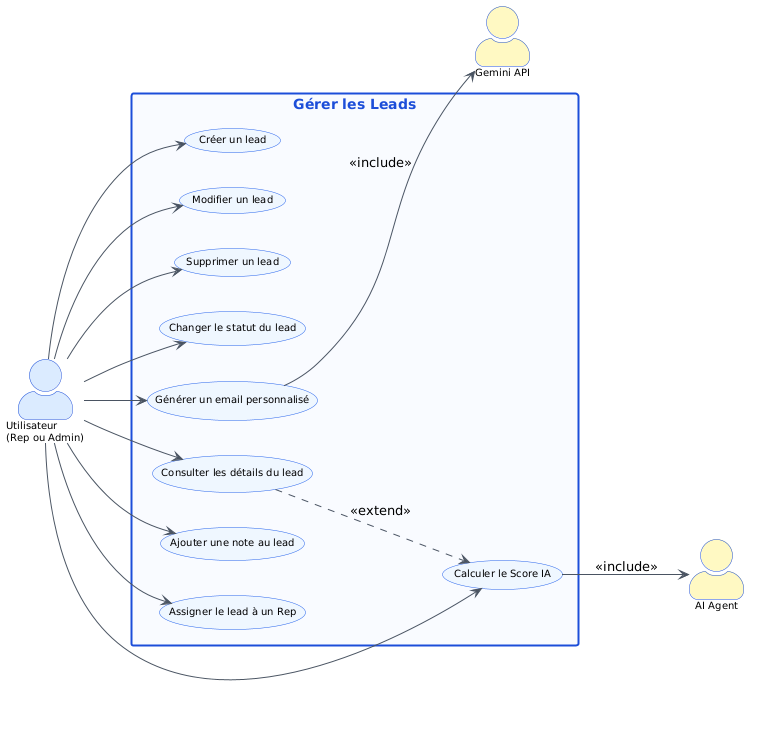
\includegraphics[width=0.8\textwidth]{images/uc_gerer_leads.png}
    \caption{Diagramme de cas d’utilisation relatif à « Gérer les Leads »}
    \label{fig:uc_gerer_leads}
\end{figure}

\subsection{Diagramme de cas d’utilisation relatif au cas d’utilisation « Importer des Données »}

Le diagramme de cas d’utilisation concernant l’« Importation de Données » est illustré à la figure 2.5. Ce cas d’utilisation, réservé à l’administrateur, détaille les étapes du processus d’importation de masse à partir d’un fichier CSV, incluant la validation de la structure du fichier, la détection de doublons et la génération d’un rapport final.

\begin{figure}[H]
    \centering
    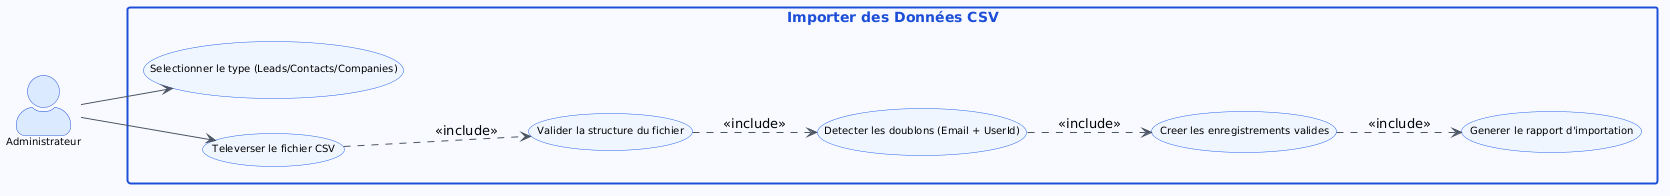
\includegraphics[width=0.8\textwidth]{images/uc_import.png}
    \caption{Diagramme de cas d’utilisation relatif à « Importer des Données »}
    \label{fig:uc_importer_donnees}
\end{figure}

\section{Diagrammes de séquence système}

Les schémas de séquence système fournissent une illustration dans l’ordre temporel des interactions entre les composants du système. Ils décrivent les interactions entre l’utilisateur, le frontend Next.js, le backend NestJS et les services tiers.

\subsection{Diagramme de séquence système relatif au cas d’utilisation « S’authentifier »}

La figure 2.6 présente le schéma du processus d’authentification d’un utilisateur. L’utilisa-
teur saisit ses informations de connexion dans le formulaire d’accès. Le backend NestJS exa-
mine l’existence du compte dans la base de données MySQL, compare le mot de passe saisi avec le hash Bcrypt enregistré, puis crée et renvoie un token JWT signé. Ce token est par la suite conservé dans les cookies sécurisés du navigateur et associé à chaque demande API sui-
vante.

\begin{figure}[H]
    \centering
    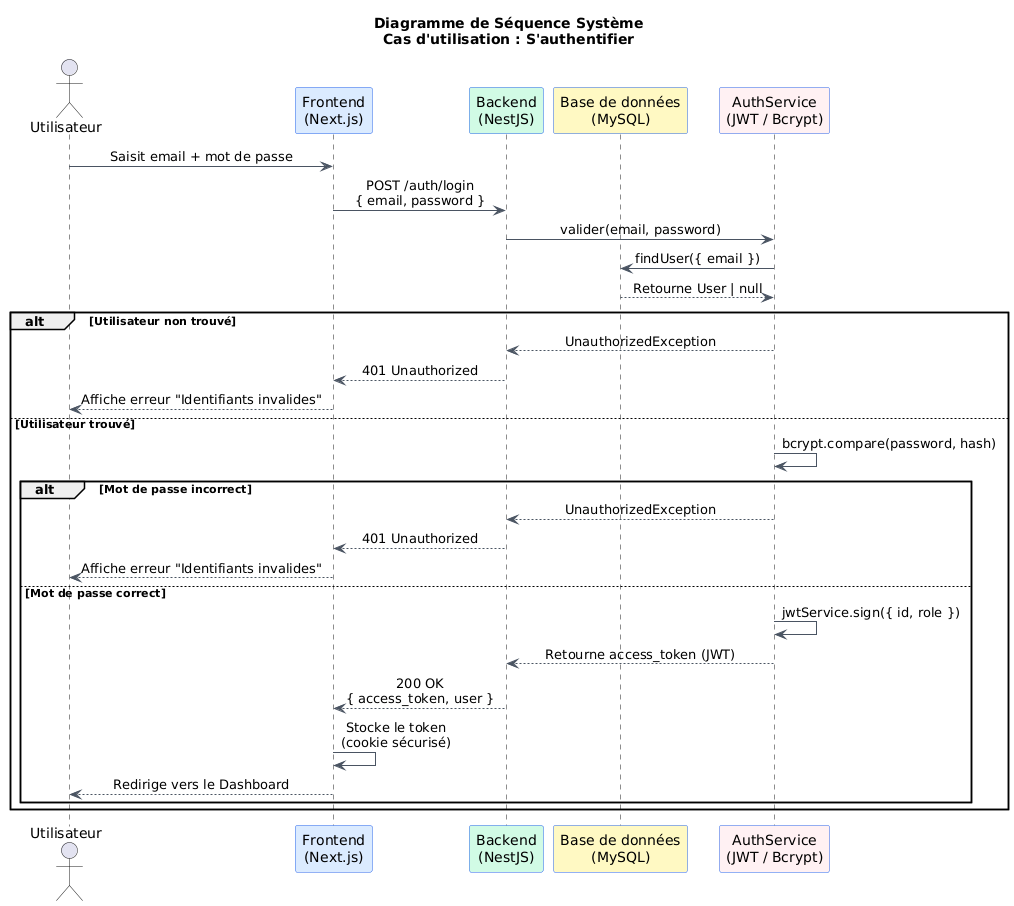
\includegraphics[width=\textwidth]{images/seq_authentification.png}
    \caption{Diagramme de séquence système relatif au cas d’utilisation « S’authentifier »}
    \label{fig:ss_authentifier}
\end{figure}

\subsection{Diagramme de séquence système relatif au cas d’utilisation « Calculer le Score IA »}

Le schéma de la figure 2.7 illustre l’interaction temporelle entre le frontend, le backend NestJS et le micro-service Python FastAPI en vue d’obtenir une prévision de conversion. Le backend puise les caractéristiques appropriées de la base de données et les transmet en POST à l’endpoint /predict-score. Si l’agent d’IA donne une réponse adéquate, le score, la catégorie ainsi que les motifs explicatifs sont sauvegardés et renvoyés à l’interface utilisateur. Si une erreur ou un dépassement de délai se produit, un score de repli calculé par le moteur des règles est renvoyé.

\begin{figure}[H]
    \centering
     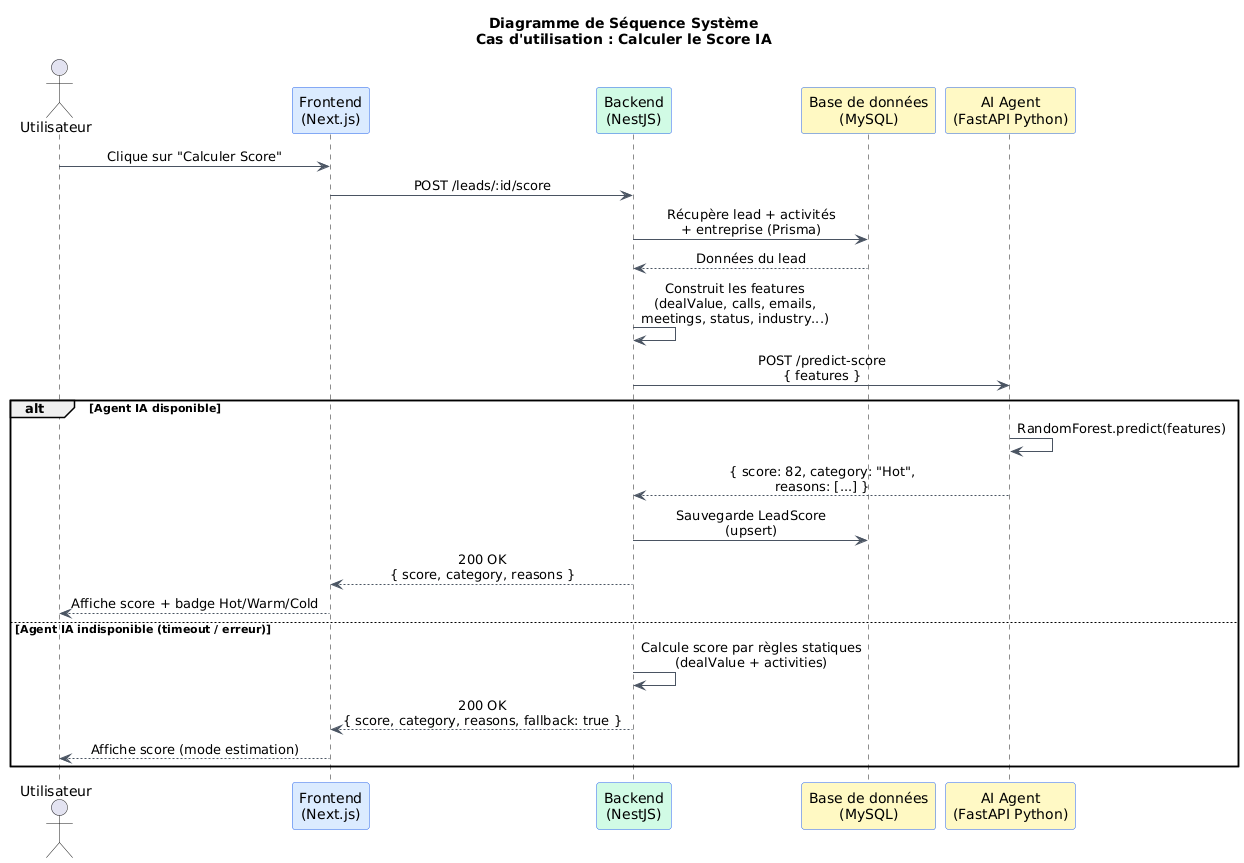
\includegraphics[width=\textwidth]{images/seq_scoring.png}
    \caption{Diagramme de séquence système relatif au cas d’utilisation « Calculer le Score IA »}
    \label{fig:ss_calculer_score_ia}
\end{figure}

\subsection{Diagramme de séquence système relatif au cas d’utilisation « Générer Email avec Gemini »}

Le schéma de la figure 2.8 représente la séquence de communication pour l’élaboration d’un projet d’email sur mesure. Le backend NestJS assemble l’intégralité du contexte du prospect (annotations, historique, évaluation IA), élabore une invite organisée pour l’API Google Gemini et restitue le contenu produit sous la forme d’un projet modifiable. En cas d’indisponibilité de l’API, le module de fallback produit un modèle sur mesure en fonction du statut et de la température du lead.

\begin{figure}[H]
    \centering
     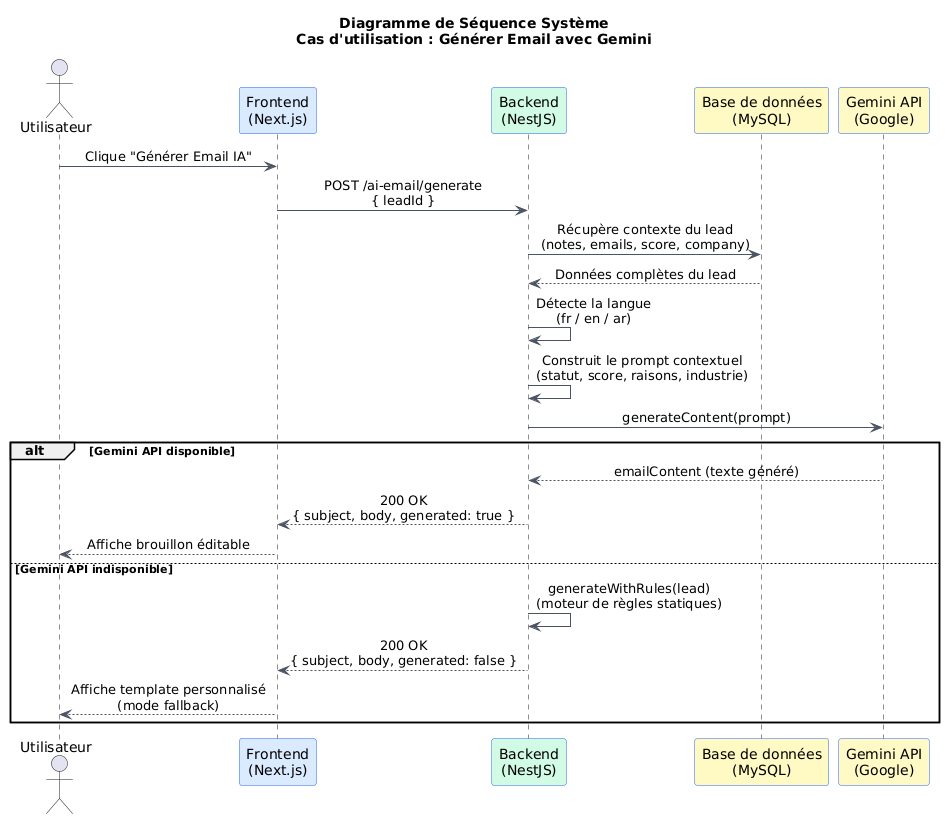
\includegraphics[width=\textwidth]{images/seq_gemini.png}
    \caption{Diagramme de séquence système relatif au cas d’utilisation « Générer Email via Gemini »}
    \label{fig:ss_generer_email}
\end{figure}

\subsection{Diagramme de séquence système relatif au cas d’utilisation « Importer des Données CSV »}

Le processus d’importation de données en grande quantité est illustré par le diagramme de la figure 2.9. Un fichier CSV est téléchargé par l’administrateur à travers l’interface. Le backend NestJS analyse le fichier, gère chaque ligne dans l’ordre en s’assurant que les champs requis sont remplis, contrôle la singularité à travers une opération d’« upset » sur la clé composite (Email + UserId) et produit un rapport final récapitulatif.

\begin{figure}[H]
    \centering
    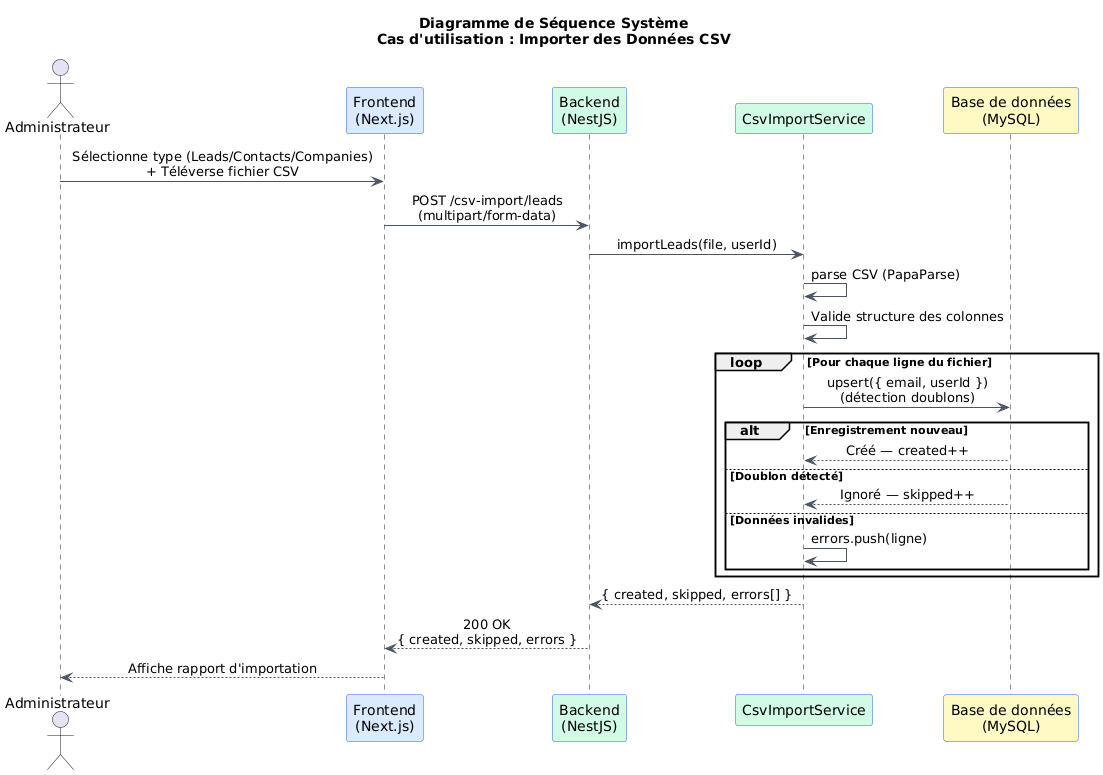
\includegraphics[width=\textwidth]{images/seq_import_csv.png}
    \caption{Diagramme de séquence système relatif au cas d’utilisation « Importer des Données CSV »}
    \label{fig:ss_importer_csv}
\end{figure}

\section*{Conclusion}

Dans ce chapitre, nous avons commencé par identifier les intervenants de notre système, à savoir le Représentant Commercial, l’Administrateur, l’API Gemini et le micro-service de scoring IA, en précisant leurs fonctions et obligations respectives. Par la suite, nous avons mi-
nutieusement défini les exigences fonctionnelles, englobant tous les modules du CRM, ainsi que les exigences non fonctionnelles liées à la sécurité, à la performance, à la disponibilité et à la facilité de maintenance. Finalement, nous avons introduit une modélisation UML organisée en packages, incluant des diagrammes de cas d’utilisation par acteur, des diagrammes détaillés par fonctionnalité et des diagrammes de séquence système relatifs aux processus critiques. Le prochain chapitre se focalisera sur la conception architecturale et les décisions technologiques prises pour l’implémentation de cette solution.